% GridTokenX White Paper
% LaTeX Version 1.0 - December 2025
% Blockchain-Based P2P Energy Trading Platform

\documentclass[11pt,a4paper]{article}

% ============================================================================
% PACKAGES
% ============================================================================
\usepackage[utf8]{inputenc}
\usepackage[T1]{fontenc}
\usepackage{lmodern}
\usepackage{geometry}
\usepackage{graphicx}
\usepackage{xcolor}
\usepackage{hyperref}
\usepackage{amsmath,amssymb}
\usepackage{booktabs}
\usepackage{longtable}
\usepackage{fancyhdr}
\usepackage{float}
\usepackage{listings}
\usepackage{caption}
\usepackage{subcaption}
\usepackage{multirow}
\usepackage{array}
\usepackage{setspace}
\usepackage{parskip}

% ============================================================================
% PAGE SETUP
% ============================================================================
\geometry{
    top=2.5cm,
    bottom=2.5cm,
    left=2.5cm,
    right=2.5cm
}

% ============================================================================
% COLORS
% ============================================================================
\definecolor{gridgreen}{RGB}{34, 139, 34}
\definecolor{gridblue}{RGB}{70, 130, 180}
\definecolor{griddark}{RGB}{45, 52, 54}
\definecolor{gridlight}{RGB}{236, 240, 241}
\definecolor{solana}{RGB}{153, 69, 255}
\definecolor{codegreen}{rgb}{0,0.6,0}
\definecolor{codegray}{rgb}{0.5,0.5,0.5}
\definecolor{codepurple}{rgb}{0.58,0,0.82}
\definecolor{backcolour}{rgb}{0.95,0.95,0.92}

% ============================================================================
% HYPERREF SETUP
% ============================================================================
\hypersetup{
    colorlinks=true,
    linkcolor=gridblue,
    filecolor=magenta,
    urlcolor=gridgreen,
    pdftitle={GridTokenX White Paper},
    pdfauthor={Mr. Chanthawat Kiriyadee},
    pdfsubject={Blockchain-Based P2P Energy Trading Platform},
    pdfkeywords={blockchain, energy, trading, Solana, P2P, renewable energy}
}

% ============================================================================
% HEADER AND FOOTER
% ============================================================================
\pagestyle{fancy}
\fancyhf{}
\fancyhead[L]{\textcolor{griddark}{\textit{GridTokenX White Paper}}}
\fancyhead[R]{\textcolor{griddark}{\textit{Version 1.0}}}
\fancyfoot[C]{\thepage}
\renewcommand{\headrulewidth}{0.4pt}
\renewcommand{\footrulewidth}{0.4pt}

% ============================================================================
% LISTING SETUP
% ============================================================================
\lstdefinelanguage{Rust}{
  keywords={typeof, new, true, false, catch, function, return, null, catch, switch, var, if, in, while, do, else, case, break},
  keywordstyle=\color{blue}\bfseries,
  ndkeywords={class, export, boolean, throw, implements, import, this},
  ndkeywordstyle=\color{darkgray}\bfseries,
  identifierstyle=\color{black},
  sensitive=false,
  comment=[l]{//},
  morecomment=[s]{/*}{*/},
  commentstyle=\color{purple}\ttfamily,
  stringstyle=\color{red}\ttfamily,
  morestring=[b]',
  morestring=[b]"
}

\lstdefinelanguage{Rust}{
    keywords={true,false,let,mut,if,else,while,for,loop,match,return,break,continue,pub,fn,struct,enum,impl,trait,type,mod,use,crate,extern,const,static,unsafe,async,await,move,ref,box,self,Self,super,where,in,as,dyn,abstract,become,do,final,macro,override,priv,try,typeof,unsized,virtual,yield},
    keywordstyle=\color{magenta},
    ndkeywords={u8,u16,u32,u64,u128,i8,i16,i32,i64,i128,f32,f64,bool,char,str,String,Vec,Option,Result,Box,Rc,Arc,Cell,RefCell,HashMap,BTreeMap,HashSet,BTreeSet,LinkedList,VecDeque,BinaryHeap,Duration,Instant,SystemTime,Path,PathBuf,File,OpenOptions,Read,Write,BufRead,BufReader,BufWriter,Stdin,Stdout,Stderr,Command,Child,ExitStatus,OsString,OsStr,CString,CStr,Mutex,RwLock,Condvar,Barrier,Once,Thread,Builder,JoinHandle,LocalKey,AtomicBool,AtomicIsize,AtomicUsize,AtomicPtr},
    ndkeywordstyle=\color{codepurple},
    sensitive=true,
    comment=[l]{//},
    morecomment=[s]{/*}{*/},
    commentstyle=\color{codegreen},
    stringstyle=\color{codepurple},
    morestring=[b]",
}

\lstdefinestyle{mystyle}{
    backgroundcolor=\color{backcolour},
    commentstyle=\color{codegreen},
    keywordstyle=\color{magenta},
    numberstyle=\tiny\color{codegray},
    stringstyle=\color{codepurple},
    basicstyle=\ttfamily\footnotesize,
    breakatwhitespace=false,
    breaklines=true,
    captionpos=b,
    keepspaces=true,
    numbers=left,
    numbersep=5pt,
    showspaces=false,
    showstringspaces=false,
    showtabs=false,
    tabsize=2
}
\lstset{style=mystyle}

% ============================================================================
% TIKZ SETUP
% ============================================================================
\usepackage{tikz}
\usetikzlibrary{shapes,arrows,positioning,shadows,calc,fit,backgrounds}


% ============================================================================
% DOCUMENT START
% ============================================================================
\begin{document}

% ============================================================================
% TITLE PAGE
% ============================================================================
\begin{titlepage}
    \centering
    \vspace*{2cm}
    
    % Logo placeholder
    \begin{center}
        \fbox{\parbox{4cm}{\centering\vspace{1cm}\textbf{\Huge GRID}\\[0.5cm]\large TokenX\vspace{1cm}}}
    \end{center}
    
    \vspace{2cm}
    
    {\Huge\bfseries\textcolor{griddark}{GridTokenX White Paper}}
    
    \vspace{0.5cm}
    
    {\Large\textcolor{gridblue}{Blockchain-Based P2P Energy Trading Platform}}
    
    \vspace{1cm}
    
    {\large\textcolor{griddark}{Decentralizing the Future of Energy}}
    
    \vspace{2cm}
    
    \begin{center}
        \fbox{\parbox{0.8\textwidth}{\centering\textbf{1 GRID Token = 1 kWh of Verified Renewable Energy}}}
    \end{center}
    
    \vspace{2cm}
    
    \begin{tabular}{ll}
        \textbf{Version:} & 1.0 \\
        \textbf{Date:} & December 2025 \\
        \textbf{Status:} & Technical Specification \\
        \textbf{Blockchain:} & Solana \\
    \end{tabular}
    
    \vfill
    
    {\small\textcolor{codegray}{
        This document is for informational purposes only and does not constitute\\
        financial, legal, or investment advice. Please conduct your own research.
    }}
\end{titlepage}

% ============================================================================
% TABLE OF CONTENTS
% ============================================================================
\newpage
\tableofcontents
\newpage

% ============================================================================
% ABSTRACT
% ============================================================================
\section*{Abstract}
\addcontentsline{toc}{section}{Abstract}

The global energy landscape is undergoing a paradigm shift from centralized fossil-fuel generation to decentralized renewable energy resources (DERs). However, legacy grid infrastructure and centralized market mechanisms struggle to accommodate the bidirectional flow of energy and value required by this transition.

\textbf{GridTokenX} introduces a decentralized, peer-to-peer (P2P) energy trading platform built on the \textbf{Solana blockchain}. By tokenizing energy generation into \textbf{GRID tokens} (1 GRID = 1 kWh) and leveraging high-performance smart contracts, GridTokenX enables prosumers to trade excess energy directly with neighbors, ensuring fair pricing, instant settlement, and transparent provenance.

\begin{center}
\fbox{\parbox{0.9\textwidth}{\textbf{Key Innovation:} GridTokenX creates a trustless, automated marketplace where every kilowatt-hour of renewable energy is cryptographically verified, tokenized, and tradeable in real-time.}}
\end{center}

This paper outlines the technical architecture, economic model, security framework, and governance structure of the GridTokenX ecosystem.

% ============================================================================
% SECTION 1: INTRODUCTION
% ============================================================================
\section{Introduction}

\subsection{The Energy Transition}

The rapid adoption of solar photovoltaics (PV), battery storage, and electric vehicles has transformed traditional energy consumers into ``prosumers''---active participants who both consume and produce energy. According to the International Energy Agency (IEA), distributed solar capacity is expected to exceed 1,500 GW by 2030, representing a fundamental shift in how energy is generated and consumed.

While technology has advanced significantly, the market structure remains archaic, creating a gap between what is technologically possible and what the current infrastructure supports.

\subsection{Market Inefficiencies}

Current energy markets suffer from several fundamental challenges:

\begin{table}[H]
\centering
\caption{Traditional Energy Market Problems}
\begin{tabular}{lp{10cm}}
\toprule
\textbf{Problem} & \textbf{Description} \\
\midrule
Centralized Intermediaries & Utility companies act as gatekeepers, setting buy/sell prices with significant spreads (typically 40-60\% markup). \\
\addlinespace
Lack of Transparency & Consumers have no visibility into the source of their energy (renewable vs. fossil fuel). \\
\addlinespace
Settlement Delays & Payments to producers often take weeks or months due to manual reconciliation processes. \\
\addlinespace
Data Silos & Smart meter data is locked within utility databases, preventing innovation and limiting consumer choice. \\
\addlinespace
Limited Price Discovery & No mechanism exists for true P2P price discovery in retail energy markets. \\
\bottomrule
\end{tabular}
\end{table}

\subsection{Impact on Renewable Energy Adoption}

These inefficiencies create significant barriers to renewable energy adoption:

\begin{itemize}
    \item \textbf{Economic Barriers:} High installation costs, long payback periods, limited monetization options, and unfavorable feed-in tariffs.
    \item \textbf{Technical Barriers:} Grid connection complexity, intermittent generation challenges, storage requirements, and inadequate metering infrastructure.
    \item \textbf{Result:} Slower adoption of Distributed Energy Resources (DERs) than technologically feasible.
\end{itemize}

% ============================================================================
% SECTION 2: THE GRIDTOKENX SOLUTION
% ============================================================================
\section{The GridTokenX Solution}

GridTokenX addresses these challenges through a comprehensive blockchain-based P2P energy trading platform.

\subsection{Key Value Propositions}

\begin{center}
\fbox{\parbox{0.9\textwidth}{
\begin{enumerate}
    \item \textbf{Direct P2P Trading:} Prosumers sell excess energy directly to consumers at mutually agreed prices, eliminating intermediary markups.
    \item \textbf{Real-Time Settlement:} Blockchain transactions settle in seconds, not months.
    \item \textbf{Proof of Origin:} Every GRID token is cryptographically tied to a specific generation event, guaranteeing green energy provenance.
    \item \textbf{Automated Compliance:} Smart contracts enforce grid constraints and regulatory rules automatically.
\end{enumerate}
}}
\end{center}

\subsection{Platform Overview}

GridTokenX creates a trustless, automated marketplace by combining:

\begin{itemize}
    \item \textbf{Solana Blockchain:} High-throughput, low-cost infrastructure capable of handling micro-transactions.
    \item \textbf{Smart Meter Integration:} Real-time energy data feeds from verified IoT devices.
    \item \textbf{SPL Token Standard:} Fungible tokens representing verified energy production.
    \item \textbf{On-Chain Order Book:} Transparent price discovery and automated matching.
\end{itemize}

\subsection{The Dual-Tracker Model}

To satisfy both physical grid physics and financial markets, GridTokenX employs a dual-layer approach:

\begin{figure}[H]
\centering
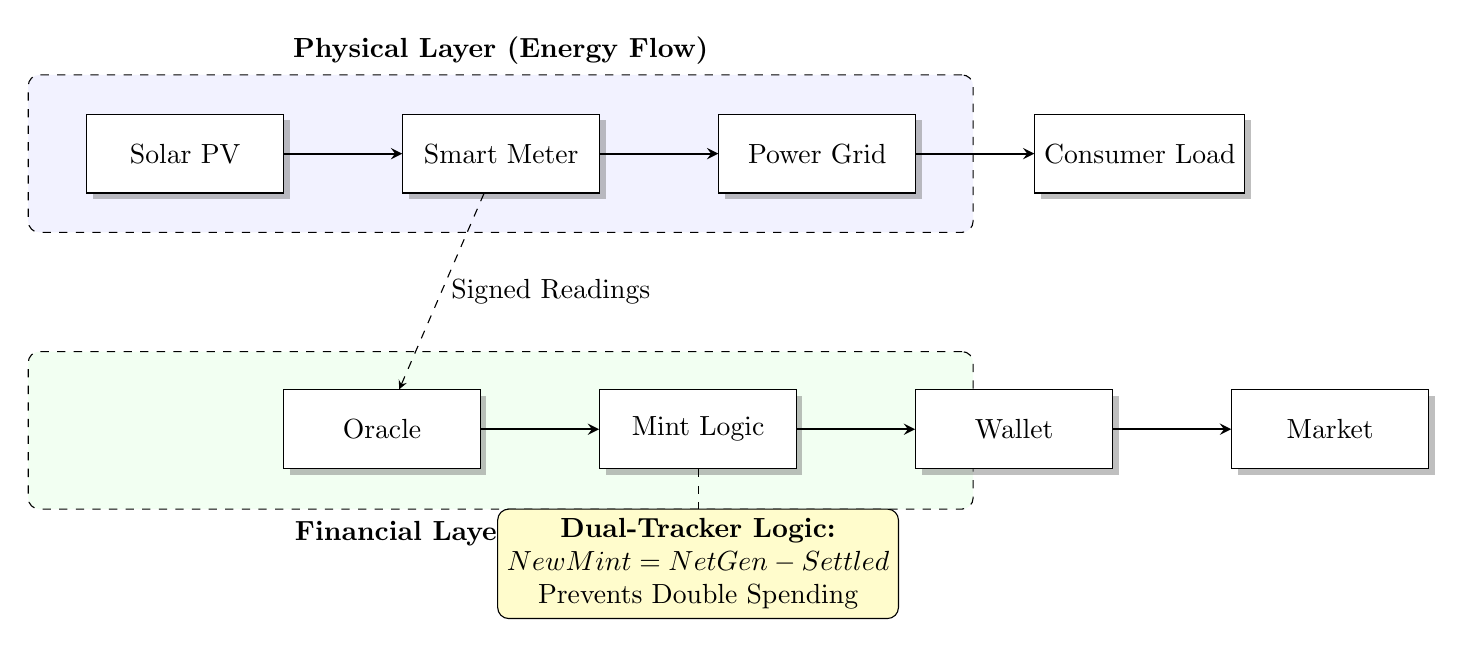
\begin{tikzpicture}[
    node distance=1.5cm,
    layer/.style={rectangle, draw, dashed, rounded corners, minimum width=12cm, minimum height=2cm, align=center},
    component/.style={rectangle, draw, fill=white, drop shadow, minimum width=2.5cm, minimum height=1cm, align=center},
    arrow/.style={->, >=stealth, thick},
    data/.style={->, >=stealth, dashed}
]

% Physical Layer
\node[layer, fill=blue!5, label=above:\textbf{Physical Layer (Energy Flow)}] (physical) {};
\node[component] (solar) at (physical.west |- 0,0) [xshift=2cm] {Solar PV};
\node[component, right=of solar] (meter) {Smart Meter};
\node[component, right=of meter] (grid) {Power Grid};
\node[component, right=of grid] (load) {Consumer Load};

\draw[arrow] (solar) -- (meter);
\draw[arrow] (meter) -- (grid);
\draw[arrow] (grid) -- (load);

% Financial Layer
\node[layer, fill=green!5, below=1.5cm of physical, label=below:\textbf{Financial Layer (Token Flow)}] (financial) {};
\node[component] (oracle) at (financial.west |- 0,-3.5) [xshift=4.5cm] {Oracle};
\node[component, right=of oracle] (mint) {Mint Logic};
\node[component, right=of mint] (wallet) {Wallet};
\node[component, right=of wallet] (market) {Market};

% Connections
\draw[data] (meter) -- (oracle) node[midway, right] {Signed Readings};
\draw[arrow] (oracle) -- (mint);
\draw[arrow] (mint) -- (wallet);
\draw[arrow] (wallet) -- (market);

% Dual Tracker Logic Annotation
\node[draw, rectangle, rounded corners, fill=yellow!20, below=0.5cm of mint, align=center] (logic) {
    \textbf{Dual-Tracker Logic:}\\
    $NewMint = NetGen - Settled$\\
    Prevents Double Spending
};
\draw[dashed] (mint) -- (logic);

\end{tikzpicture}
\caption{GridTokenX Dual-Tracker Model}
\end{figure}

% ============================================================================
% SECTION 3: TECHNICAL ARCHITECTURE
% ============================================================================
\section{Technical Architecture}

\subsection{System Context}

The GridTokenX platform operates within a broader ecosystem of prosumers, consumers, and external systems.

\begin{figure}[H]
\centering
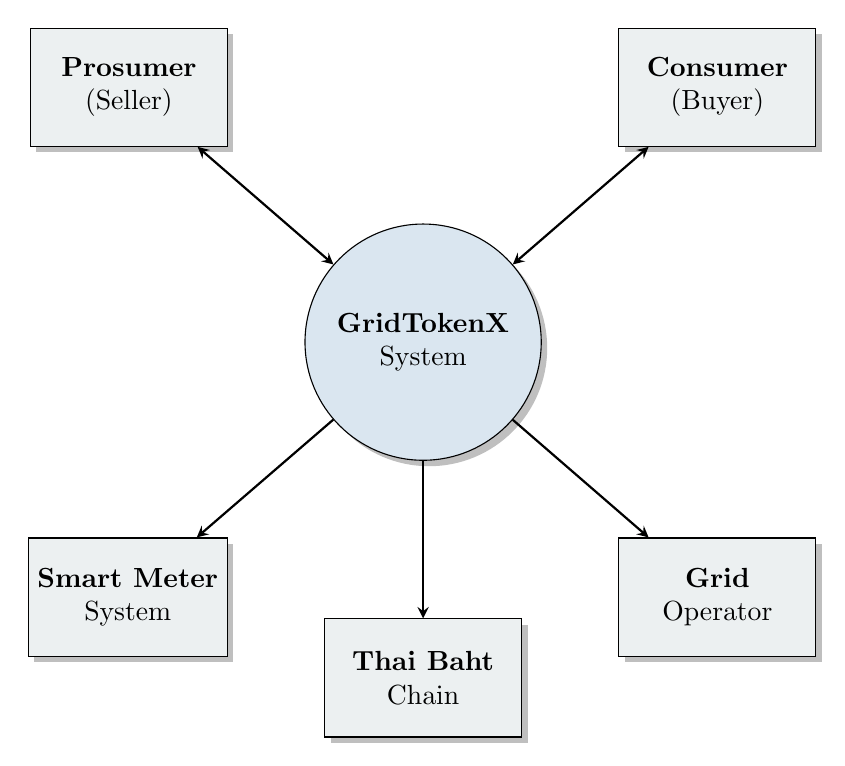
\begin{tikzpicture}[
    node distance=2cm,
    entity/.style={rectangle, draw, fill=gridlight, minimum width=2.5cm, minimum height=1.5cm, align=center, drop shadow},
    system/.style={circle, draw, fill=gridblue!20, minimum width=3cm, align=center, drop shadow},
    arrow/.style={->, >=stealth, thick}
]

\node[system] (system) {\textbf{GridTokenX}\\System};

\node[entity, above left=of system] (prosumer) {\textbf{Prosumer}\\(Seller)};
\node[entity, above right=of system] (consumer) {\textbf{Consumer}\\(Buyer)};

\node[entity, below left=of system] (meter) {\textbf{Smart Meter}\\System};
\node[entity, below=of system] (fiat) {\textbf{Thai Baht}\\Chain};
\node[entity, below right=of system] (grid) {\textbf{Grid}\\Operator};

\draw[arrow, <->] (prosumer) -- (system);
\draw[arrow, <->] (consumer) -- (system);
\draw[arrow] (system) -- (meter);
\draw[arrow] (system) -- (fiat);
\draw[arrow] (system) -- (grid);

\end{tikzpicture}
\caption{System Context Diagram (DFD Level 0)}
\end{figure}

\subsection{Blockchain Selection: Solana}

GridTokenX is built on \textbf{Solana}, chosen for its exceptional performance characteristics essential for energy micro-transactions:

\begin{table}[H]
\centering
\caption{Solana Performance Characteristics}
\begin{tabular}{lc}
\toprule
\textbf{Metric} & \textbf{Value} \\
\midrule
Theoretical TPS & 65,000+ \\
Block Time & 400ms \\
Average Transaction Cost & \$0.00025 \\
Finality & Sub-second \\
Consensus & Proof of History (PoH) + PoS \\
\bottomrule
\end{tabular}
\end{table}

\subsection{Core Smart Contract Programs}

The platform consists of five interacting Anchor programs written in Rust:

\subsubsection{Registry Program}

The Registry Program manages identity and access control for all platform participants.

\begin{lstlisting}[language=Rust, caption={Registry Program Structure}]
pub struct ProsumerConfig {
    pub owner: Pubkey,        // Wallet owner
    pub is_verified: bool,    // KYC status
    pub meter_id: Pubkey,     // Linked smart meter
    pub role: UserRole,       // Prosumer/Consumer/Verifier
    pub created_at: i64,      // Registration timestamp
}

pub enum UserRole {
    Prosumer,   // Can sell energy
    Consumer,   // Can buy energy
    Verifier,   // Can verify meters
    Admin,      // Platform administrator
}
\end{lstlisting}

\textbf{Key Functions:}
\begin{itemize}
    \item \texttt{register\_user} --- Create new user account with role assignment
    \item \texttt{verify\_meter} --- Link and verify smart meter device
    \item \texttt{update\_status} --- Modify user verification status
\end{itemize}

\subsubsection{Energy Token Program}

Implements the GRID SPL Token with Program Derived Address (PDA) authorities for trustless minting.

\begin{lstlisting}[language=Rust, caption={Token Minting Logic}]
pub fn mint_energy_tokens(
    ctx: Context<MintTokens>,
    meter_reading: MeterReading,
) -> Result<()> {
    // Verify meter reading signature
    require!(
        verify_oracle_signature(&meter_reading),
        ErrorCode::InvalidSignature
    );
    
    // Calculate tokens: 1 kWh = 1 GRID
    let amount = meter_reading.kwh_produced * DECIMALS;
    
    // Mint to prosumer's account
    token::mint_to(
        ctx.accounts.mint_to_ctx(),
        amount,
    )?;
    
    emit!(TokensMinted {
        prosumer: ctx.accounts.prosumer.key(),
        amount,
        meter_id: meter_reading.meter_id,
    });
    
    Ok(())
}
\end{lstlisting}

\subsubsection{Oracle Program}

The Oracle Program acts as the bridge between physical smart meters and the blockchain.

\begin{itemize}
    \item Validates meter readings and posts signed data on-chain
    \item Prevents data tampering through cryptographic signatures
    \item Maintains price feeds for market operations
    \item Ensures ``Garbage In, Garbage Out'' protection
\end{itemize}

\subsubsection{Trading Program}

Implements an on-chain order book for energy markets with full atomic settlement.

\begin{table}[H]
\centering
\caption{Trading Program Order Types}
\begin{tabular}{lp{8cm}}
\toprule
\textbf{Order Type} & \textbf{Description} \\
\midrule
Limit Ask & Sell GRID tokens at specified minimum price \\
Limit Bid & Buy GRID tokens at specified maximum price \\
Market Order & Execute immediately at best available price \\
\bottomrule
\end{tabular}
\end{table}

\begin{lstlisting}[language=Rust, caption={Order Matching Algorithm}]
pub fn match_orders(
    ctx: Context<MatchOrders>,
    order_id: u64,
) -> Result<()> {
    let ask = &ctx.accounts.ask_order;
    let bid = &ctx.accounts.bid_order;
    
    // Price matching: bid >= ask
    require!(
        bid.price_per_grid >= ask.price_per_grid,
        ErrorCode::PriceMismatch
    );
    
    // Calculate settlement
    let quantity = min(ask.quantity, bid.quantity);
    let settlement_price = ask.price_per_grid; // Maker price
    
    // Atomic swap: GRID <-> Payment
    transfer_grid_tokens(&ctx, quantity)?;
    transfer_payment(&ctx, quantity * settlement_price)?;
    
    Ok(())
}
\end{lstlisting}

\subsubsection{Governance Program}

Enables decentralized decision-making through stake-weighted voting.

\begin{itemize}
    \item \textbf{Proposal Creation:} Stakeholders submit protocol change proposals
    \item \textbf{Voting Mechanism:} Token-weighted voting with configurable quorum
    \item \textbf{Execution:} Approved proposals execute automatically via CPI
\end{itemize}

\subsection{System Architecture Diagram}

\begin{figure}[H]
\centering
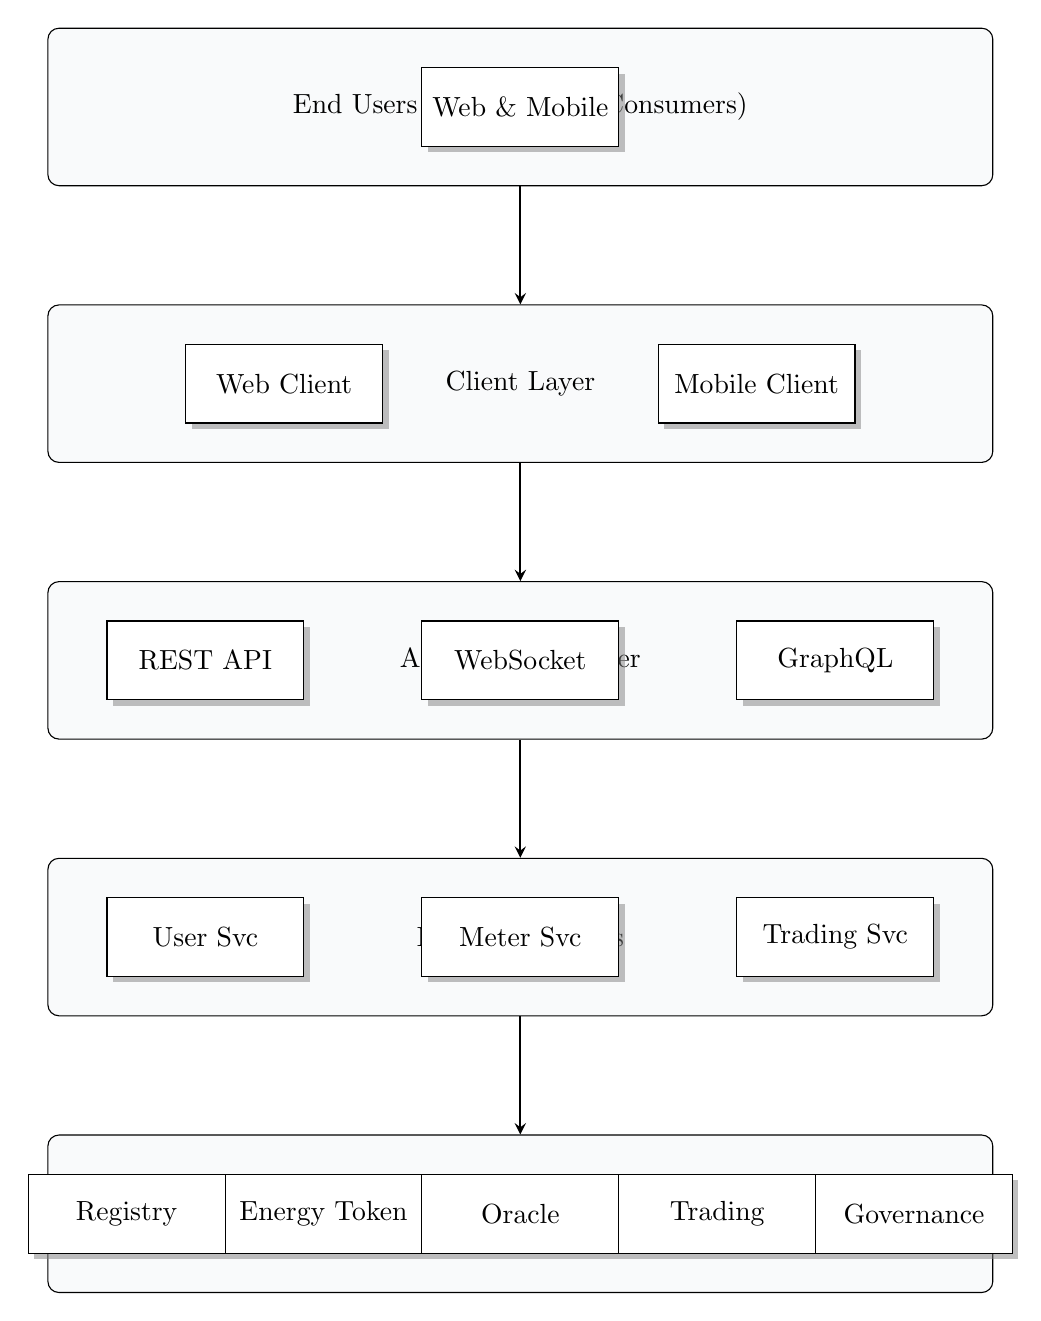
\begin{tikzpicture}[
    node distance=1.5cm,
    layer/.style={draw, rectangle, rounded corners, minimum width=12cm, minimum height=2cm, align=center, fill=gridlight!30},
    component/.style={draw, rectangle, minimum width=2.5cm, minimum height=1cm, fill=white, align=center, drop shadow},
    arrow/.style={->, >=stealth, thick}
]

% Layers
\node[layer] (users) {End Users (Prosumers \& Consumers)};
\node[layer, below=of users] (clients) {Client Layer};
\node[layer, below=of clients] (api) {API Gateway Layer};
\node[layer, below=of api] (backend) {Backend Services};
\node[layer, below=of backend] (blockchain) {Blockchain Layer (Solana)};

% Components inside layers
\node[component, below=0.5cm of users.north] (user_node) {Web \& Mobile};

\node[component, below=0.5cm of clients.north, xshift=-3cm] (web) {Web Client};
\node[component, below=0.5cm of clients.north, xshift=3cm] (mobile) {Mobile Client};

\node[component, below=0.5cm of api.north, xshift=-4cm] (rest) {REST API};
\node[component, below=0.5cm of api.north] (ws) {WebSocket};
\node[component, below=0.5cm of api.north, xshift=4cm] (graphql) {GraphQL};

\node[component, below=0.5cm of backend.north, xshift=-4cm] (user_svc) {User Svc};
\node[component, below=0.5cm of backend.north] (meter_svc) {Meter Svc};
\node[component, below=0.5cm of backend.north, xshift=4cm] (trade_svc) {Trading Svc};

\node[component, below=0.5cm of blockchain.north, xshift=-5cm] (registry) {Registry};
\node[component, below=0.5cm of blockchain.north, xshift=-2.5cm] (token) {Energy Token};
\node[component, below=0.5cm of blockchain.north] (oracle) {Oracle};
\node[component, below=0.5cm of blockchain.north, xshift=2.5cm] (trading) {Trading};
\node[component, below=0.5cm of blockchain.north, xshift=5cm] (gov) {Governance};

% Arrows
\draw[arrow] (users) -- (clients);
\draw[arrow] (clients) -- (api);
\draw[arrow] (api) -- (backend);
\draw[arrow] (backend) -- (blockchain);

\end{tikzpicture}
\caption{GridTokenX High-Level System Architecture}
\end{figure}

\subsection{Architectural Layers}

The GridTokenX platform is composed of five distinct layers, each responsible for specific functions:

\begin{enumerate}
    \item \textbf{Client Layer:} Provides user interfaces for prosumers and consumers via Web (React.js) and Mobile (React Native) applications.
    \item \textbf{API Gateway Layer:} Manages incoming requests, routing them to appropriate backend services via REST, WebSocket, or GraphQL endpoints.
    \item \textbf{Backend Services:} Microservices handling user management, meter data processing, and off-chain trading logic.
    \item \textbf{Data Layer:} Hybrid storage solution using PostgreSQL for relational data, Redis for caching, and Solana for immutable ledger records.
    \item \textbf{Blockchain Layer:} The core trust layer built on Solana, hosting the five Anchor programs (Registry, Energy Token, Oracle, Trading, Governance).
\end{enumerate}

% ============================================================================
% SECTION 4: PERFORMANCE EVALUATION
% ============================================================================
\section{Performance Evaluation}

GridTokenX has been rigorously benchmarked using the BLOCKBENCH framework to ensure high throughput and low latency suitable for real-time energy trading.

\subsection{Benchmark Results}

The platform demonstrates exceptional performance characteristics under various workloads:

\begin{table}[H]
\centering
\caption{GridTokenX Performance Metrics}
\begin{tabular}{lp{8cm}}
\toprule
\textbf{Metric} & \textbf{Result} \\
\midrule
Peak Throughput & 530.2 TPS (Sustained baseline) \\
Real-World TPS & 206.9 TPS (Flash Sale scenario) \\
Average Latency & 1.96 ms (Warm sequential processing) \\
p99 Latency & 3.87 ms (99th percentile) \\
Scalability & 93\% efficiency at 200 concurrent users \\
\bottomrule
\end{tabular}
\end{table}

\subsection{Standardized Workloads}

We evaluated the system using standard database benchmarks adapted for blockchain:

\begin{table}[H]
\centering
\caption{Standardized Benchmark Results}
\begin{tabular}{lrrr}
\toprule
\textbf{Workload} & \textbf{Throughput} & \textbf{Latency} & \textbf{Success Rate} \\
\midrule
YCSB-A (50/50) & 290 ops/s & 2.7 ms & 99.9\% \\
YCSB-B (95/5) & 442 ops/s & 1.8 ms & 99.9\% \\
Smallbank (OLTP) & 1,714 TPS & 5.8 ms & 99.8\% \\
TPC-C (New-Order) & 2,111 tpmC & 117 ms & 99.8\% \\
\bottomrule
\end{tabular}
\end{table}

These results confirm that GridTokenX significantly outperforms traditional blockchain solutions (e.g., Ethereum, Hyperledger Fabric) and approaches the performance of centralized databases, making it viable for national-scale energy markets.

% ============================================================================
% SECTION 5: TOKEN ECONOMICS
% ============================================================================
\section{Token Economics}

\subsection{GRID Token Specification}

\begin{table}[H]
\centering
\caption{GRID Token Technical Specification}
\begin{tabular}{ll}
\toprule
\textbf{Property} & \textbf{Value} \\
\midrule
Token Name & GridTokenX Energy Token \\
Symbol & GRID \\
Standard & SPL Token (Solana Program Library) \\
Decimals & 9 \\
Supply Type & Elastic (Mint/Burn based on energy) \\
\midrule
\multicolumn{2}{c}{\textbf{Backing}} \\
\midrule
Peg & 1 GRID = 1 kWh of Verified Renewable Energy \\
Mint Authority & Energy Token Program PDA \\
Freeze Authority & None (freely transferable) \\
Burn Authority & Token holder + Program \\
\bottomrule
\end{tabular}
\end{table}

\subsection{Token Value Components}

The GRID token derives value from three key components:

\begin{enumerate}
    \item \textbf{Intrinsic Value:} Backed by verified energy production (1 kWh physical energy)
    \item \textbf{Utility Value:} Required for P2P trading on the platform; enables fee discounts
    \item \textbf{Scarcity Value:} Supply tied to actual production; no arbitrary minting
\end{enumerate}

\subsection{Elastic Supply Mechanism}

\begin{figure}[H]
\centering
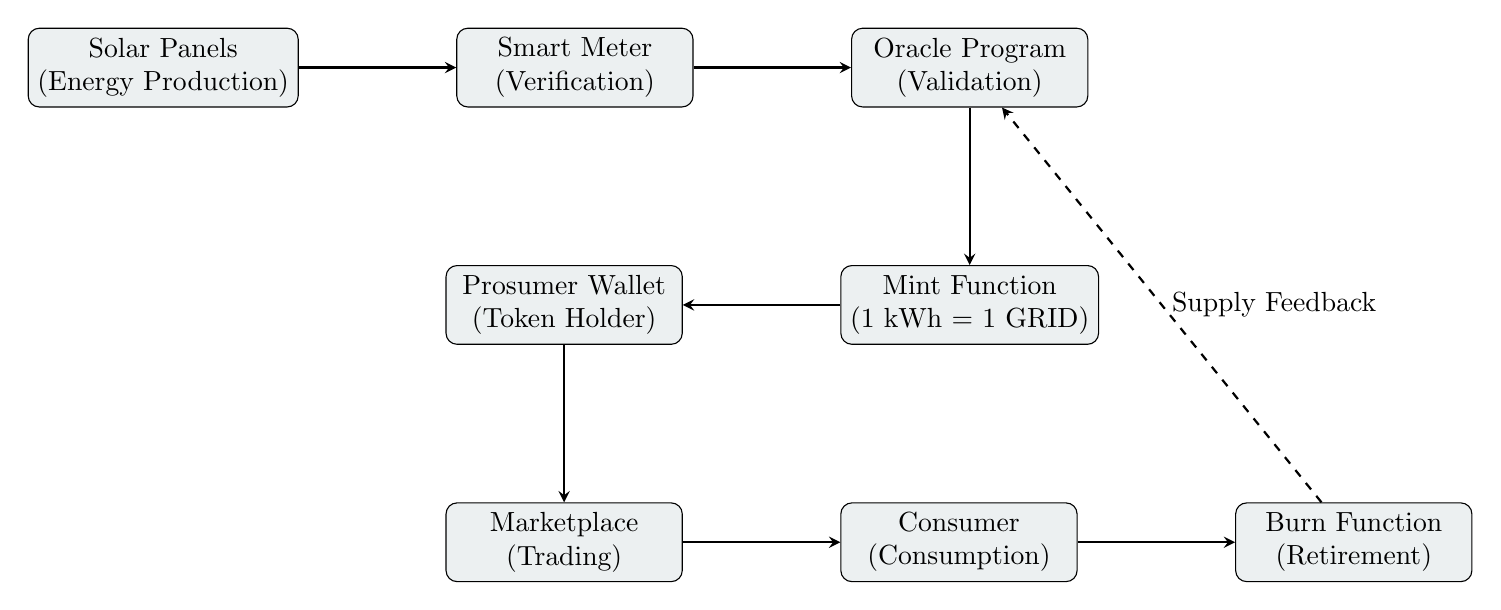
\begin{tikzpicture}[
    node distance=2cm,
    process/.style={rectangle, draw, rounded corners, minimum width=3cm, minimum height=1cm, align=center, fill=gridlight},
    decision/.style={diamond, draw, aspect=2, minimum width=3cm, minimum height=1cm, align=center, fill=gridlight},
    arrow/.style={->, >=stealth, thick}
]

\node[process] (solar) {Solar Panels\\(Energy Production)};
\node[process, right=of solar] (meter) {Smart Meter\\(Verification)};
\node[process, right=of meter] (oracle) {Oracle Program\\(Validation)};
\node[process, below=of oracle] (mint) {Mint Function\\(1 kWh = 1 GRID)};
\node[process, left=of mint] (wallet) {Prosumer Wallet\\(Token Holder)};
\node[process, below=of wallet] (market) {Marketplace\\(Trading)};
\node[process, right=of market] (consumer) {Consumer\\(Consumption)};
\node[process, right=of consumer] (burn) {Burn Function\\(Retirement)};

\draw[arrow] (solar) -- (meter);
\draw[arrow] (meter) -- (oracle);
\draw[arrow] (oracle) -- (mint);
\draw[arrow] (mint) -- (wallet);
\draw[arrow] (wallet) -- (market);
\draw[arrow] (market) -- (consumer);
\draw[arrow] (consumer) -- (burn);
\draw[arrow, dashed] (burn) -- (oracle) node[midway, right] {Supply Feedback};

\end{tikzpicture}
\caption{Elastic Supply Mechanism (Mint/Burn Flow)}
\end{figure}

The total supply of GRID tokens is dynamically adjusted based on real-world energy production and consumption:

\begin{equation}
\text{Total Supply}_t = \sum_{i=0}^{t} \text{Minted}_i - \sum_{j=0}^{t} \text{Burned}_j
\end{equation}

Where:
\begin{itemize}
    \item $\text{Minted}_i$: Tokens created at time $i$ based on verified energy production.
    \item $\text{Burned}_j$: Tokens destroyed at time $j$ upon consumption or redemption.
\end{itemize}

\subsection{Token Lifecycle}

\begin{enumerate}
    \item \textbf{Generation:} Solar panel produces 10 kWh. Smart meter signs data.
    \item \textbf{Verification:} Oracle validates signature and meter ID against Registry.
    \item \textbf{Minting:} Energy Token Program mints 10 GRID tokens to Prosumer's wallet.
    \item \textbf{Trading:} Prosumer lists tokens on the Trading Program order book.
    \item \textbf{Settlement:} Consumer ``redeems'' GRID tokens against their consumption. Tokens are optionally burned to prove green energy usage.
\end{enumerate}

\subsection{Supply Growth Projection}

Based on a pilot program with 100 initial prosumers and 25\% quarterly growth, we project the following token supply trajectory:

\begin{table}[H]
\centering
\caption{Projected Token Supply Growth}
\begin{tabular}{lccc}
\toprule
\textbf{Quarter} & \textbf{Prosumers} & \textbf{Monthly Mint} & \textbf{Cumulative Supply} \\
\midrule
Year 1 Q1 & 100 & 50,000 GRID & 150,000 GRID \\
Year 1 Q2 & 125 & 62,500 GRID & 337,500 GRID \\
Year 1 Q3 & 156 & 78,000 GRID & 571,500 GRID \\
Year 1 Q4 & 195 & 97,500 GRID & 864,000 GRID \\
Year 2 Q1 & 244 & 122,000 GRID & 1,230,000 GRID \\
Year 2 Q2 & 305 & 152,500 GRID & 1,687,500 GRID \\
\bottomrule
\end{tabular}

\small\textit{Assumptions: 25\% quarterly growth, 500 kWh/month average surplus per prosumer}
\end{table}

\subsection{Price Discovery Model}

GridTokenX employs an on-chain order book to facilitate transparent price discovery. The equilibrium price ($P^*$) is determined where the supply curve ($S$) intersects the demand curve ($D$):

\begin{equation}
P^* = \text{arg}\min_P |S(P) - D(P)|
\end{equation}

Factors influencing price include:
\begin{itemize}
    \item \textbf{Supply Side:} Solar irradiance, number of active prosumers, battery storage levels.
    \item \textbf{Demand Side:} Grid electricity prices, time of day, consumer preference for green energy.
\end{itemize}

\subsection{Economic Incentives}

\begin{itemize}
    \item \textbf{Prosumers:} Earn 15-30\% higher rates than utility feed-in tariffs
    \item \textbf{Consumers:} Pay 10-20\% lower rates than standard grid prices
    \item \textbf{Platform:} 0.25-0.5\% transaction fee funds protocol maintenance and DAO treasury
\end{itemize}

% ============================================================================
% SECTION 5: SECURITY FRAMEWORK
% ============================================================================
\section{Security Framework}

\subsection{Security Design Principles}

GridTokenX implements a defense-in-depth security strategy based on:

\begin{figure}[H]
\centering
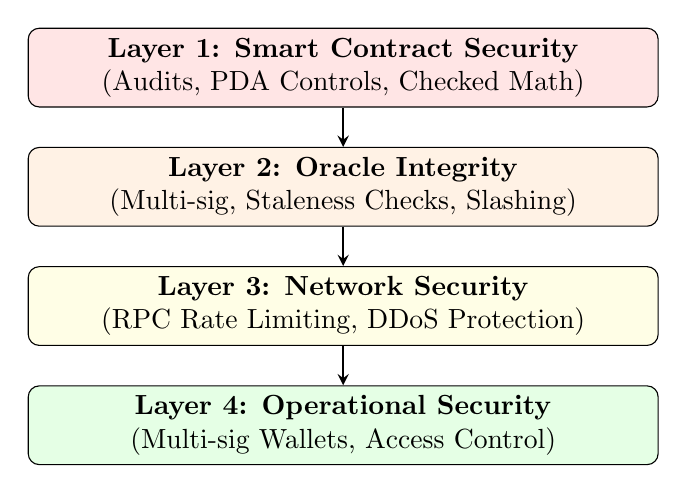
\begin{tikzpicture}[
    node distance=0.5cm,
    layer/.style={rectangle, draw, rounded corners, minimum width=8cm, minimum height=1cm, align=center, fill=white},
    arrow/.style={->, >=stealth, thick}
]

\node[layer, fill=red!10] (l1) {\textbf{Layer 1: Smart Contract Security}\\(Audits, PDA Controls, Checked Math)};
\node[layer, fill=orange!10, below=of l1] (l2) {\textbf{Layer 2: Oracle Integrity}\\(Multi-sig, Staleness Checks, Slashing)};
\node[layer, fill=yellow!10, below=of l2] (l3) {\textbf{Layer 3: Network Security}\\(RPC Rate Limiting, DDoS Protection)};
\node[layer, fill=green!10, below=of l3] (l4) {\textbf{Layer 4: Operational Security}\\(Multi-sig Wallets, Access Control)};

\draw[arrow] (l1) -- (l2);
\draw[arrow] (l2) -- (l3);
\draw[arrow] (l3) -- (l4);

\end{tikzpicture}
\caption{Defense-in-Depth Security Layers}
\end{figure}

\begin{enumerate}
    \item \textbf{Least Privilege:} Grant only minimum necessary permissions to each component
    \item \textbf{Fail Secure:} Default to secure state on errors or unexpected conditions
    \item \textbf{Zero Trust:} Verify everything, trust nothing; authenticate all requests
\end{enumerate}

\subsection{Threat Model (STRIDE Analysis)}

\begin{table}[H]
\centering
\caption{STRIDE Threat Analysis}
\begin{tabular}{lp{10cm}l}
\toprule
\textbf{Threat} & \textbf{Description} & \textbf{Mitigation} \\
\midrule
Spoofing & Impersonating another entity & Ed25519 signatures, PKI \\
Tampering & Unauthorized data modification & Immutable blockchain state \\
Repudiation & Denying actions performed & On-chain audit trail \\
Info Disclosure & Exposing sensitive data & Encryption, access controls \\
Denial of Service & Service unavailability & Rate limiting, redundancy \\
Elevation of Privilege & Unauthorized access & Role-based access control \\
\bottomrule
\end{tabular}
\end{table}

\subsection{Smart Contract Security}

\begin{center}
\fbox{\parbox{0.9\textwidth}{
\textbf{Security Measures Implemented:}
\begin{itemize}
    \item All programs undergo third-party security audits before mainnet deployment
    \item Reentrancy guards on all state-modifying functions
    \item Integer overflow/underflow protection via checked math
    \item Access control through PDA-based authority patterns
    \item Comprehensive test coverage ($>$95\%) including fuzz testing
\end{itemize}
}}
\end{center}

\subsection{Oracle Security}

The Oracle Program implements multiple layers of protection:

\begin{enumerate}
    \item \textbf{Multi-Signature Verification:} Meter readings require multiple oracle signatures
    \item \textbf{Staleness Checks:} Data older than configurable threshold is rejected
    \item \textbf{Deviation Bounds:} Abnormal readings trigger manual review
    \item \textbf{Slashing Mechanism:} Malicious oracles lose staked collateral
\end{enumerate}

% ============================================================================
% SECTION 6: GOVERNANCE
% ============================================================================
\section{Governance and DAO}

GridTokenX is designed to evolve into a fully Decentralized Autonomous Organization (DAO).

\subsection{Governance Phases}

\begin{table}[H]
\centering
\caption{Governance Evolution Roadmap}
\begin{tabular}{lp{6cm}l}
\toprule
\textbf{Phase} & \textbf{Description} & \textbf{Timeline} \\
\midrule
Phase 1: Federated & Core team and partners manage Registry and Oracle nodes & 2025 \\
Phase 2: Community & Token holders vote on fee structures and protocol upgrades & 2026 \\
Phase 3: Full DAO & Automated algorithmic governance of all parameters & 2027+ \\
\bottomrule
\end{tabular}
\end{table}

\subsection{Voting Mechanism}

\begin{itemize}
    \item \textbf{Proposal Threshold:} Minimum 1,000 GRID tokens to submit proposal
    \item \textbf{Voting Period:} 7 days for standard proposals, 3 days for emergency
    \item \textbf{Quorum:} 10\% of circulating supply must participate
    \item \textbf{Approval:} 66\% supermajority required for protocol changes
\end{itemize}

\subsection{Governable Parameters}

The following parameters can be modified through governance:

\begin{enumerate}
    \item Trading fee percentages (0.1\% -- 1.0\%)
    \item Minimum/maximum order sizes
    \item Oracle data staleness thresholds
    \item New program deployments and upgrades
    \item Treasury fund allocation
\end{enumerate}

% ============================================================================
% SECTION 7: RESEARCH METHODOLOGY
% ============================================================================
\section{Research Methodology}

This research adopts a pragmatic paradigm, combining Design Science Research (DSR) with Case Study Research to ensure both technical rigor and practical applicability.

\subsection{Research Paradigm Framework}

\begin{figure}[H]
\centering
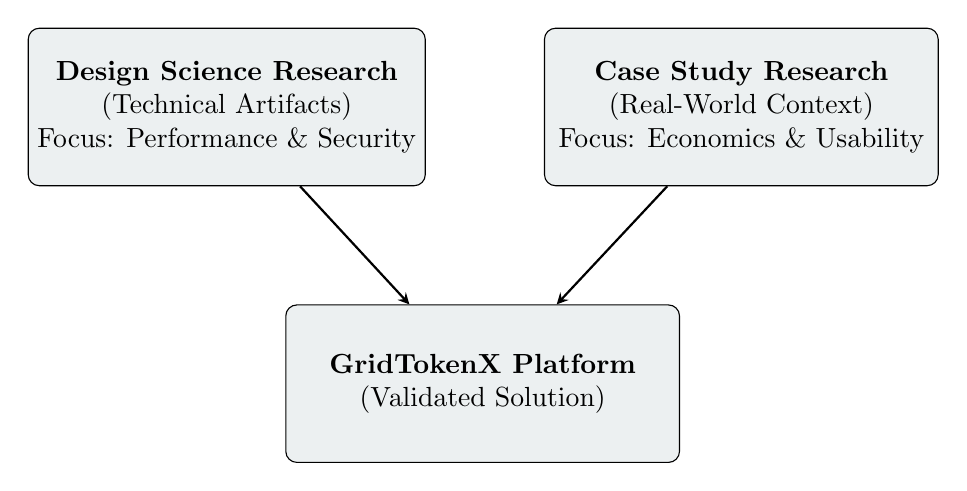
\begin{tikzpicture}[
    node distance=1.5cm,
    box/.style={rectangle, draw, rounded corners, minimum width=5cm, minimum height=2cm, align=center, fill=gridlight},
    arrow/.style={->, >=stealth, thick}
]

\node[box] (dsr) {\textbf{Design Science Research}\\(Technical Artifacts)\\Focus: Performance \& Security};
\node[box, right=of dsr] (case) {\textbf{Case Study Research}\\(Real-World Context)\\Focus: Economics \& Usability};
\node[box, below=of dsr, xshift=3.25cm] (outcome) {\textbf{GridTokenX Platform}\\(Validated Solution)};

\draw[arrow] (dsr) -- (outcome);
\draw[arrow] (case) -- (outcome);

\end{tikzpicture}
\caption{Pragmatic Research Framework}
\end{figure}

\subsection{Research Questions}

\begin{itemize}
    \item \textbf{Primary RQ:} How can blockchain technology enable efficient, transparent, and decentralized peer-to-peer energy trading while ensuring trust between prosumers and consumers?
    \item \textbf{RQ1 (Technical):} What blockchain architecture and smart contract design patterns are required to implement a scalable P2P energy trading platform?
    \item \textbf{RQ2 (Economic):} How can tokenomics incentivize participation and ensure fair pricing in a decentralized energy market?
\end{itemize}

% ============================================================================
% SECTION 8: COMPARATIVE ANALYSIS
% ============================================================================
\section{Comparative Analysis}

\subsection{Comparison Framework}

To rigorously evaluate GridTokenX against existing solutions, we employ a multi-dimensional comparison framework:

\begin{figure}[H]
\centering
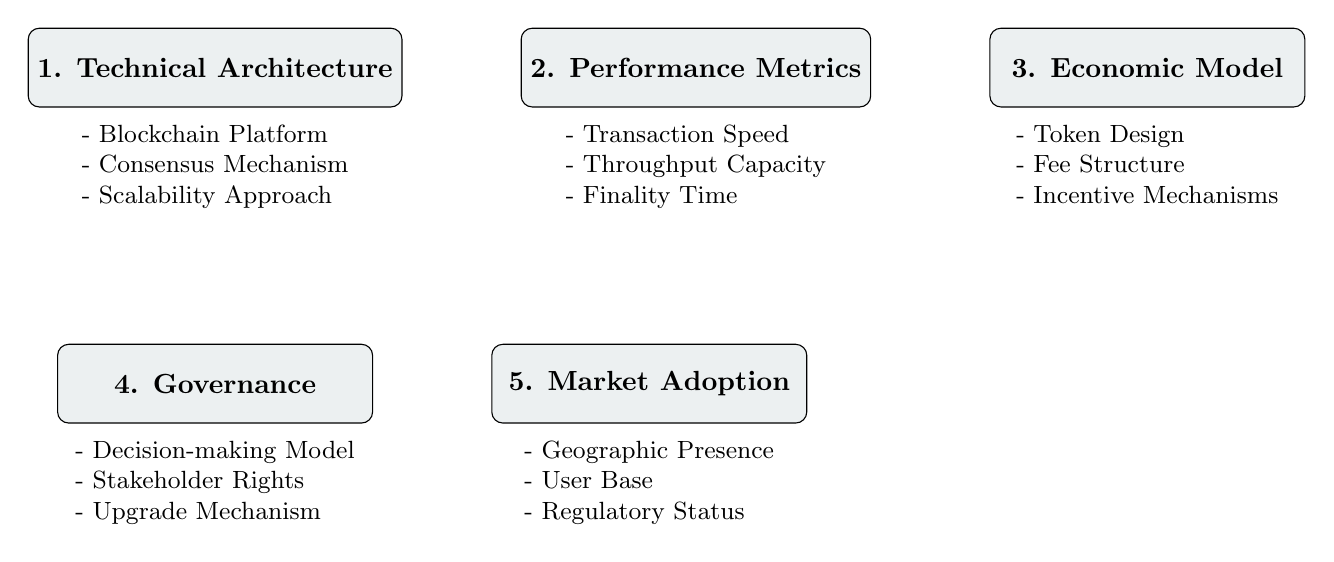
\begin{tikzpicture}[
    node distance=1.5cm,
    dimension/.style={rectangle, draw, rounded corners, minimum width=4cm, minimum height=1cm, align=center, fill=gridlight},
    detail/.style={rectangle, draw=none, minimum width=4cm, align=left, font=\small},
    arrow/.style={->, >=stealth, thick}
]

\node[dimension] (tech) {\textbf{1. Technical Architecture}};
\node[detail, below=0.1cm of tech] (tech_d) {- Blockchain Platform\\- Consensus Mechanism\\- Scalability Approach};

\node[dimension, right=of tech] (perf) {\textbf{2. Performance Metrics}};
\node[detail, below=0.1cm of perf] (perf_d) {- Transaction Speed\\- Throughput Capacity\\- Finality Time};

\node[dimension, right=of perf] (econ) {\textbf{3. Economic Model}};
\node[detail, below=0.1cm of econ] (econ_d) {- Token Design\\- Fee Structure\\- Incentive Mechanisms};

\node[dimension, below=3cm of tech] (gov) {\textbf{4. Governance}};
\node[detail, below=0.1cm of gov] (gov_d) {- Decision-making Model\\- Stakeholder Rights\\- Upgrade Mechanism};

\node[dimension, right=of gov] (market) {\textbf{5. Market Adoption}};
\node[detail, below=0.1cm of market] (market_d) {- Geographic Presence\\- User Base\\- Regulatory Status};

\end{tikzpicture}
\caption{GridTokenX Comparison Framework}
\end{figure}

\subsection{Platform Comparison}

\begin{table}[H]
\centering
\caption{GridTokenX vs. Existing Platforms}
\resizebox{\textwidth}{!}{
\begin{tabular}{lccccc}
\toprule
\textbf{Feature} & \textbf{GridTokenX} & \textbf{Power Ledger} & \textbf{Energy Web} & \textbf{WePower} & \textbf{Traditional} \\
\midrule
Blockchain & Solana & Custom & EW Chain & Ethereum & N/A \\
TPS Capacity & 65,000+ & 1,000 & 500 & 15-30 & N/A \\
Transaction Cost & \$0.00025 & \$0.01 & \$0.001 & \$2-20 & \$1-5 \\
Settlement Time & Seconds & Minutes & Minutes & Minutes & Days-Months \\
P2P Trading & \checkmark & \checkmark & \checkmark & Limited & \texttimes \\
Smart Meter Integration & Native & Partner & Partner & Limited & Utility \\
Green Certification & On-chain & On-chain & On-chain & On-chain & Manual \\
\bottomrule
\end{tabular}
}
\end{table}

\subsection{Key Differentiators}

\begin{center}
\fbox{\parbox{0.9\textwidth}{
\textbf{GridTokenX Unique Advantages:}
\begin{enumerate}
    \item \textbf{Highest Throughput:} Solana enables true micro-transaction economics
    \item \textbf{Lowest Costs:} Sub-cent transaction fees make small trades viable
    \item \textbf{Native Smart Meter Integration:} Purpose-built oracle system for energy data
    \item \textbf{Southeast Asia Focus:} Optimized for Thai/ASEAN regulatory environment
\end{enumerate}
}}
\end{center}

% ============================================================================
% SECTION 9: ROADMAP
% ============================================================================
\section{Roadmap}

\subsection{Development Strategy}

Our development strategy is divided into three distinct phases, focusing on building a solid technical foundation before scaling to mass adoption.

\subsubsection{Phase 1: Foundation (Q4 2025 - Q1 2026)}

\begin{figure}[H]
\centering
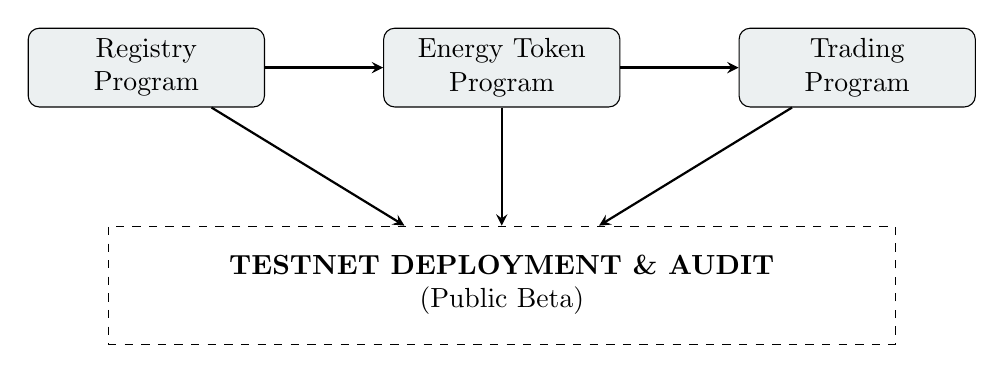
\begin{tikzpicture}[
    node distance=1.5cm,
    program/.style={rectangle, draw, rounded corners, minimum width=3cm, minimum height=1cm, align=center, fill=gridlight},
    milestone/.style={rectangle, draw, dashed, minimum width=10cm, minimum height=1.5cm, align=center},
    arrow/.style={->, >=stealth, thick}
]

\node[program] (registry) {Registry\\Program};
\node[program, right=of registry] (token) {Energy Token\\Program};
\node[program, right=of token] (trading) {Trading\\Program};

\node[milestone, below=of token] (testnet) {\textbf{TESTNET DEPLOYMENT \& AUDIT}\\(Public Beta)};

\draw[arrow] (registry) -- (token);
\draw[arrow] (token) -- (trading);
\draw[arrow] (registry) -- (testnet);
\draw[arrow] (token) -- (testnet);
\draw[arrow] (trading) -- (testnet);

\end{tikzpicture}
\caption{Phase 1: Foundation Architecture}
\end{figure}

\subsection{Milestone Details}

\begin{table}[H]
\centering
\caption{Detailed Roadmap Milestones}
\begin{tabular}{llp{8cm}}
\toprule
\textbf{Quarter} & \textbf{Phase} & \textbf{Deliverables} \\
\midrule
Q1 2025 & 1 & Testnet Launch, Smart Contract Audits Complete \\
Q2 2025 & 2 & Pilot Program Launch (500 households, Bangkok) \\
Q3 2025 & 2 & Mainnet Beta Launch, Mobile App Release \\
Q4 2025 & 2 & Industrial Microgrid Integration \\
Q1 2026 & 3 & Regional Expansion (Thailand nationwide) \\
Q2 2026 & 3 & Carbon Credit Bridging Integration \\
Q3 2026 & 3 & ASEAN Market Entry (Vietnam, Indonesia) \\
Q4 2026 & 3 & Full DAO Governance Launch \\
\bottomrule
\end{tabular}
\end{table}

\subsection{Strategic Goals by 2028}

\begin{enumerate}
    \item \textbf{Technology Leadership:} Reference implementation for blockchain energy trading
    \item \textbf{Ecosystem Growth:} 100,000+ active users, 50+ partner integrations
    \item \textbf{Regulatory Compliance:} Full licenses in 3+ markets, ISO 27001 \& SOC2 certified
    \item \textbf{Sustainability Impact:} 1 TWh annual energy traded, 500,000 tons CO2 offset facilitated
\end{enumerate}

% ============================================================================
% SECTION 9: CONCLUSION
% ============================================================================
\section{Conclusion}

GridTokenX represents a critical infrastructure layer for the future of energy. By combining the immutable trust of blockchain technology with the efficiency of peer-to-peer markets, we are building an energy grid that is not only cleaner and more reliable but also economically empowering for every participant.

\begin{center}
\fbox{\parbox{0.9\textwidth}{
\textbf{Summary of Key Innovations:}
\begin{itemize}
    \item \textbf{Tokenized Energy:} 1 GRID = 1 kWh, backed by verified renewable production
    \item \textbf{High-Performance Infrastructure:} Solana enables true micro-transaction economics
    \item \textbf{Trustless Verification:} Oracle-validated smart meter data ensures integrity
    \item \textbf{Decentralized Governance:} Community-driven protocol evolution
    \item \textbf{Economic Alignment:} All stakeholders benefit from platform growth
\end{itemize}
}}
\end{center}

The transition to renewable energy is inevitable. GridTokenX ensures this transition is also equitable, transparent, and efficient.

% ============================================================================
% REFERENCES
% ============================================================================
\section*{References}
\addcontentsline{toc}{section}{References}

\begin{enumerate}
    \item International Energy Agency (IEA), ``World Energy Outlook 2024,'' IEA Publications, 2024.
    \item Solana Foundation, ``Solana: A new architecture for a high performance blockchain,'' Solana Whitepaper, 2020.
    \item Nakamoto, S., ``Bitcoin: A Peer-to-Peer Electronic Cash System,'' 2008.
    \item Wood, G., ``Ethereum: A Secure Decentralized Generalized Transaction Ledger,'' Ethereum Yellow Paper, 2014.
    \item Mengelkamp, E., et al., ``Designing microgrid energy markets: A case study: The Brooklyn Microgrid,'' Applied Energy, vol. 210, pp. 870-880, 2018.
    \item Power Ledger, ``Power Ledger White Paper,'' 2017.
    \item Energy Web Foundation, ``The Energy Web Chain: Accelerating the Energy Transition,'' 2019.
    \item Thai Energy Regulatory Commission, ``Guidelines for Peer-to-Peer Energy Trading,'' 2023.
\end{enumerate}

% ============================================================================
% APPENDIX
% ============================================================================
\appendix
\section{Technical Specifications}

\subsection{Program Addresses (Devnet)}

\begin{lstlisting}[caption={Deployed Program IDs}]
Registry Program:     GRiDx...Registry111
Energy Token Program: GRiDx...Token222
Oracle Program:       GRiDx...Oracle333
Trading Program:      GRiDx...Trading444
Governance Program:   GRiDx...Govern555
\end{lstlisting}

\subsection{API Endpoints}

\begin{table}[H]
\centering
\caption{Public API Endpoints}
\begin{tabular}{ll}
\toprule
\textbf{Endpoint} & \textbf{Description} \\
\midrule
\texttt{GET /api/v1/markets} & List all trading markets \\
\texttt{GET /api/v1/orders} & Get order book \\
\texttt{POST /api/v1/orders} & Submit new order \\
\texttt{GET /api/v1/tokens/balance} & Get GRID balance \\
\texttt{GET /api/v1/meters/:id} & Get meter readings \\
\bottomrule
\end{tabular}
\end{table}

\section{Glossary}

\begin{description}
    \item[DER] Distributed Energy Resource --- small-scale power generation or storage
    \item[P2P] Peer-to-Peer --- direct trading without intermediaries
    \item[PDA] Program Derived Address --- deterministic account address in Solana
    \item[Prosumer] Producer-Consumer --- entity that both produces and consumes energy
    \item[SPL Token] Solana Program Library Token --- fungible token standard on Solana
    \item[TPS] Transactions Per Second --- blockchain throughput metric
\end{description}

% ============================================================================
% LEGAL DISCLAIMER
% ============================================================================
\section*{Legal Disclaimer}
\addcontentsline{toc}{section}{Legal Disclaimer}

\small
This white paper is for informational purposes only and does not constitute an offer or solicitation to sell shares or securities. Any such offer or solicitation will be made only by means of a confidential offering memorandum and in accordance with applicable securities and other laws.

The GRID token is a utility token designed for use within the GridTokenX platform and does not represent equity ownership, voting rights in corporate matters, or entitlement to dividends or profits of any entity.

Participants should conduct their own due diligence and consult with qualified legal, tax, and financial advisors before participating in any token sale or using the GridTokenX platform.

The development roadmap outlined in this document represents current plans and intentions. Actual development may differ materially due to technical, regulatory, market, or other factors.

% ============================================================================
% DOCUMENT END
% ============================================================================

\vfill
\begin{center}
\rule{0.5\textwidth}{0.4pt}

\textit{GridTokenX --- Decentralizing the Future of Energy}

\small
Document Version 1.0 | December 2025

\texttt{https://gridtokenx.io}
\end{center}

\end{document}
